%----------------------------------------------------------------------------------------
%	DESARROLLO (40-45 hojas)
%----------------------------------------------------------------------------------------

\pagestyle{empty}
\chapter {Desarrollo}

El principal objetivo del trabajo es implementar un algoritmo que aporte seis grados de libertad a vídeo e imagen para realidad virtual y que se pueda ejecutar consumiendo la menor cantidad de recursos posibles. Para poder tratar este planteamiento en tiempo real es necesario utilizar herramientas de aceleración por \textit{hardware}.

Las tecnologías que se van a explorar para los diferentes métodos son las siguientes:

\begin{itemize}
\item Unity como motor de desarrollo por ser de ámbito profesional y multiplataforma.
\item \textit{Shaders} gráficos como herramienta que permita la explotación de la GPU mediante técnicas clásicas de gráficos.
\item \textit{Shaders} de cómputo como herramienta alternativa a los \textit{shaders} gráficos por la versatilidad que proporcionan.
\item \textit{Visual Studio} como entorno de edición y depuración de código por la cantidad de \textit{plugins} disponibles.
\end{itemize}

\section{El entorno de desarrollo}

Los motores gráficos y de videojuegos son una herramienta para agilizar el desarrollo de demos y de aplicaciones multiplataforma. Unity se encarga de proporcionar la infraestructura necesaria para poder centrarse en el desarrollo específico del proyecto. Los principales elementos a utilizar serán:

\begin{itemize}
\item Las escenas se podrían definir como el contenedor global de objetos, cámaras y luces.
\item Los GameObject son todos los elementos que pueden ser metidos en una escena y sus componentes que son la manera de añadirles lógica mediante el lenguaje de programación C	\# .
\item Las cámaras que son GameObjects especializados en obtener imágenes del entorno tridimensional y que pueden convertirse en cámaras de realidad virtual.
\end{itemize}

\subsection{Shaders Gráficos}
Los \textit{shaders} gráficos configuran la \textit{pipeline} gráfica, que tiene la función de recibir una representación de la escena tridimensional como entrada y generar una imagen bidimensional como salida. 

Son una de las partes de la infraestructura de Unity y se configuran mediante unos elementos llamados materiales.

Existen diferentes maneras de programar los \textit{shaders} gráficos, entre las cuales se ha decidido utilizar los métodos de modificación de vértices y fragmentos, por tener experiencia previa utilizándolos y ofrecer lo necesario para el desarrollo.

\subsection{Shaders de cómputo}
Los \textit{shaders} de cómputo surgieron como respuesta a los desarrolladores que utilizaban los \textit{shaders} gráficos con un propósito general para aprovechar la capacidad de cálculo de la tarjeta gráfica.

Unity también proporciona maneras de utilizar estos \textit{shaders} y al contrario que los anteriores, no están sujetos a una \textit{pipeline}, sino que pueden ser utilizados en cualquier momento.

Estos \textit{shaders}, al utilizar la GPU al igual que los gráficos pueden hacer uso, si así se les indica, de recursos de manera compartida. Esta funcionalidad es importante porque será utilizada durante el desarrollo.


\section{Metodología}
La metodología utilizada en el desarrollo se ha basado en \textit{Scrum}, proponiendo pequeños \textit{sprint} una vez terminado el anterior. Se podrían clasificar estos sprint en tres grupos:

\begin{itemize}
\item Investigación, cuya motivación era el descubrimiento de tecnologías utilizadas por otros desarrolladores para conseguir mejorar los resultados ,tanto en calidad como en rendimiento.
\item Implementación de nuevos algoritmos o mejoras de los ya existentes, habitualmente, en función de lo investigado.
\item Evaluación de la validez de la implementación y poner de manifiesto los problemas que deben ser solucionados.
\end{itemize}

Como las implementaciones son diferentes entre ellas y se han realizado muchas pruebas, se van a ir comentando los resultados en cada iteración, en lugar de comentarlos todos al final.

Las pruebas se realizan en un ordenador de sobremesa con un procesador i7-7700K, una tarjeta gráfica Nvidia Geforce GTX1070 y 16 GB de RAM.

\section{Generación de imágenes con las que trabajar}
Con la finalidad de tener un entorno de pruebas controlado y fiable, se ha montado una escena con contenido gratuito del \textit{Asset Store}. Las principales características buscadas eran un entorno con suficientes elementos con una buena distribución, que el entorno fuera complejo y que los tamaños de los objetos fueran coherentes. Finalmente se eligió el paquete ``Sci-Fi Styled Modular Pack'' (disponible en ``\url{https://assetstore.unity.com/packages/3d/environments/sci-fi/sci-fi-styled-modular-pack-82913}'') y se estableció la cámara como indican las fotos \ref{fig:camera-position} y \ref{fig:camera-position-2}.

\begin{figure}[H]
\centering
\begin{subfigure}{.47\linewidth}
	\centering
  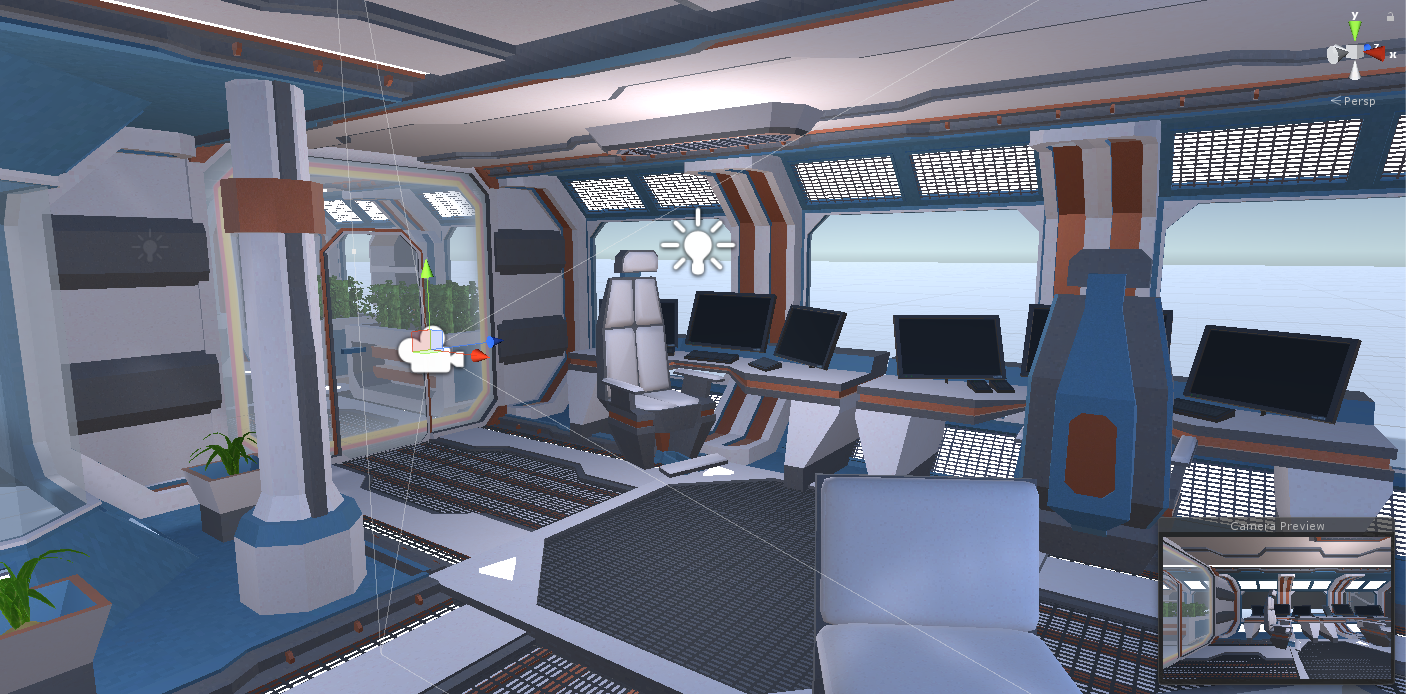
\includegraphics[width=\textwidth]{camera-position}
  \caption{Posición desde un punto de vista.}
  \label{fig:camera-position}
\end{subfigure}%
\hspace{.05\linewidth}
\begin{subfigure}{.47\linewidth}
	\centering
  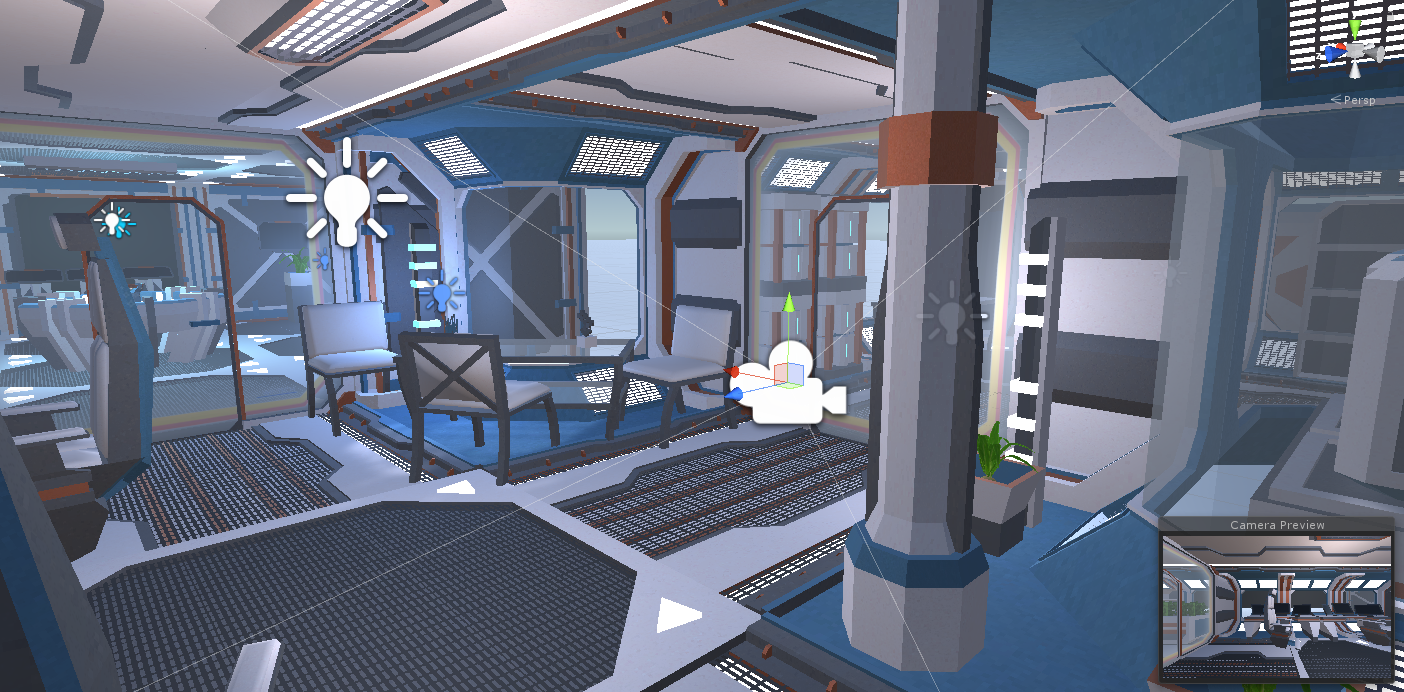
\includegraphics[width=\textwidth]{camera-position-2}
  \caption{Posición desde otro punto de vista.}
  \label{fig:camera-position-2}
\end{subfigure}
\caption{Posición de la cámara para captar imágenes estéreo 360º.}
\end{figure}
\FloatBarrier

Esta posición se ha elegido por varias razones. La primera es por la silla en los escritorios y la columna situada detrás de la cámara. Son objetos bastante cercanos con otros elementos detrás de ellos, lo que permite comprobar si el desplazamiento con los 6 grados de libertad es correcto y se produce paralaje. 

A la derecha de la cámara hay un pasillo con muchas líneas en el suelo que sirven para verificar que las líneas del suelo no se deforman. Además hay cristales para ver como se comporta el algoritmo en ese caso.

Una vez elegido el entorno para trabajar, se procede a capturar una imagen estéreo 360º. Para ello se utiliza una característica de las cámaras de Unity llamada \texttt{RenderToCubemap} y que permite capturar \textit{Cubemaps} basándose en el algoritmo de \textit{Google ODS} ya mencionado en el ``Estado del arte'' y disponible en \cite{GoogleStereoscopy}. Este procedimiento hay que repetirlo una vez por cada ojo para obtener una imagen estéreo correcta. Esta característica proporciona dos \textit{Cubemaps} y deben ser convertidos a una textura equirectangular estereoscópica \textit{top/down}. Una vez hecho, se codifica en un archivo de imagen PNG.

Por otro lado se necesita el mapa de profundidad estereoscópico que se consigue con un procedimiento parecido, pero con una serie de pasos previos que preparen la escena y restableciendo el estado anterior al final del \textit{render}. Primero y más importante hay que construir un \textit{shader} que pinte la profundidad, para ello hay diferentes maneras de hacerlo de las cuales se han probado dos:

\begin{itemize}
\item La primera que se implementó consiste en codificar la profundidad en las cuatro componentes de la imagen con la función que proporciona Unity llamada ``\texttt{EncodeFloatRGBA}''. Este método se abandonó por aumentar la complejidad y el ruido ante posibles errores a la hora de desarrollar. Se puede ver un ejemplo en \ref{fig:float-encoded-depthmap-example}.
\item Por otro lado la profundidad podía ser guardada como un solo número, y ante esto existía la posibilidad de utilizar una textura de \textit{•} con el formato ``\texttt{RFloat}'' que equivale a un único número en coma floatante de 32 bit por cada píxel, o una textura ``\texttt{ARGB32}'' habitual y guardarlo en una de sus componentes. Se optó finalmente, por compatibilidad con diferentes plataformas, por la segunda forma guardando la profundidad en la componente roja. Se puede ver un ejemplo en \ref{fig:red-depthmap-encoded-example}.
\end{itemize}


\begin{figure}[H]
  \centering
  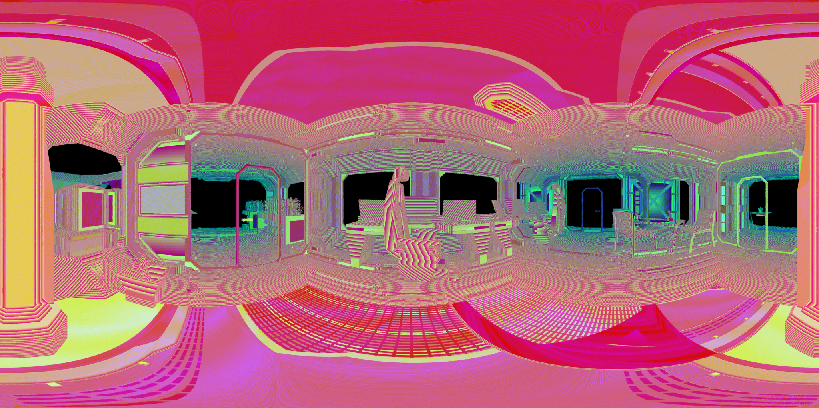
\includegraphics[width=0.7\textwidth]{float-encoded-depthmap}
  \caption{Mapa de profundidad codificado a float.}
  \label{fig:float-encoded-depthmap-example}
\end{figure}

\begin{figure}[H]
  \centering
  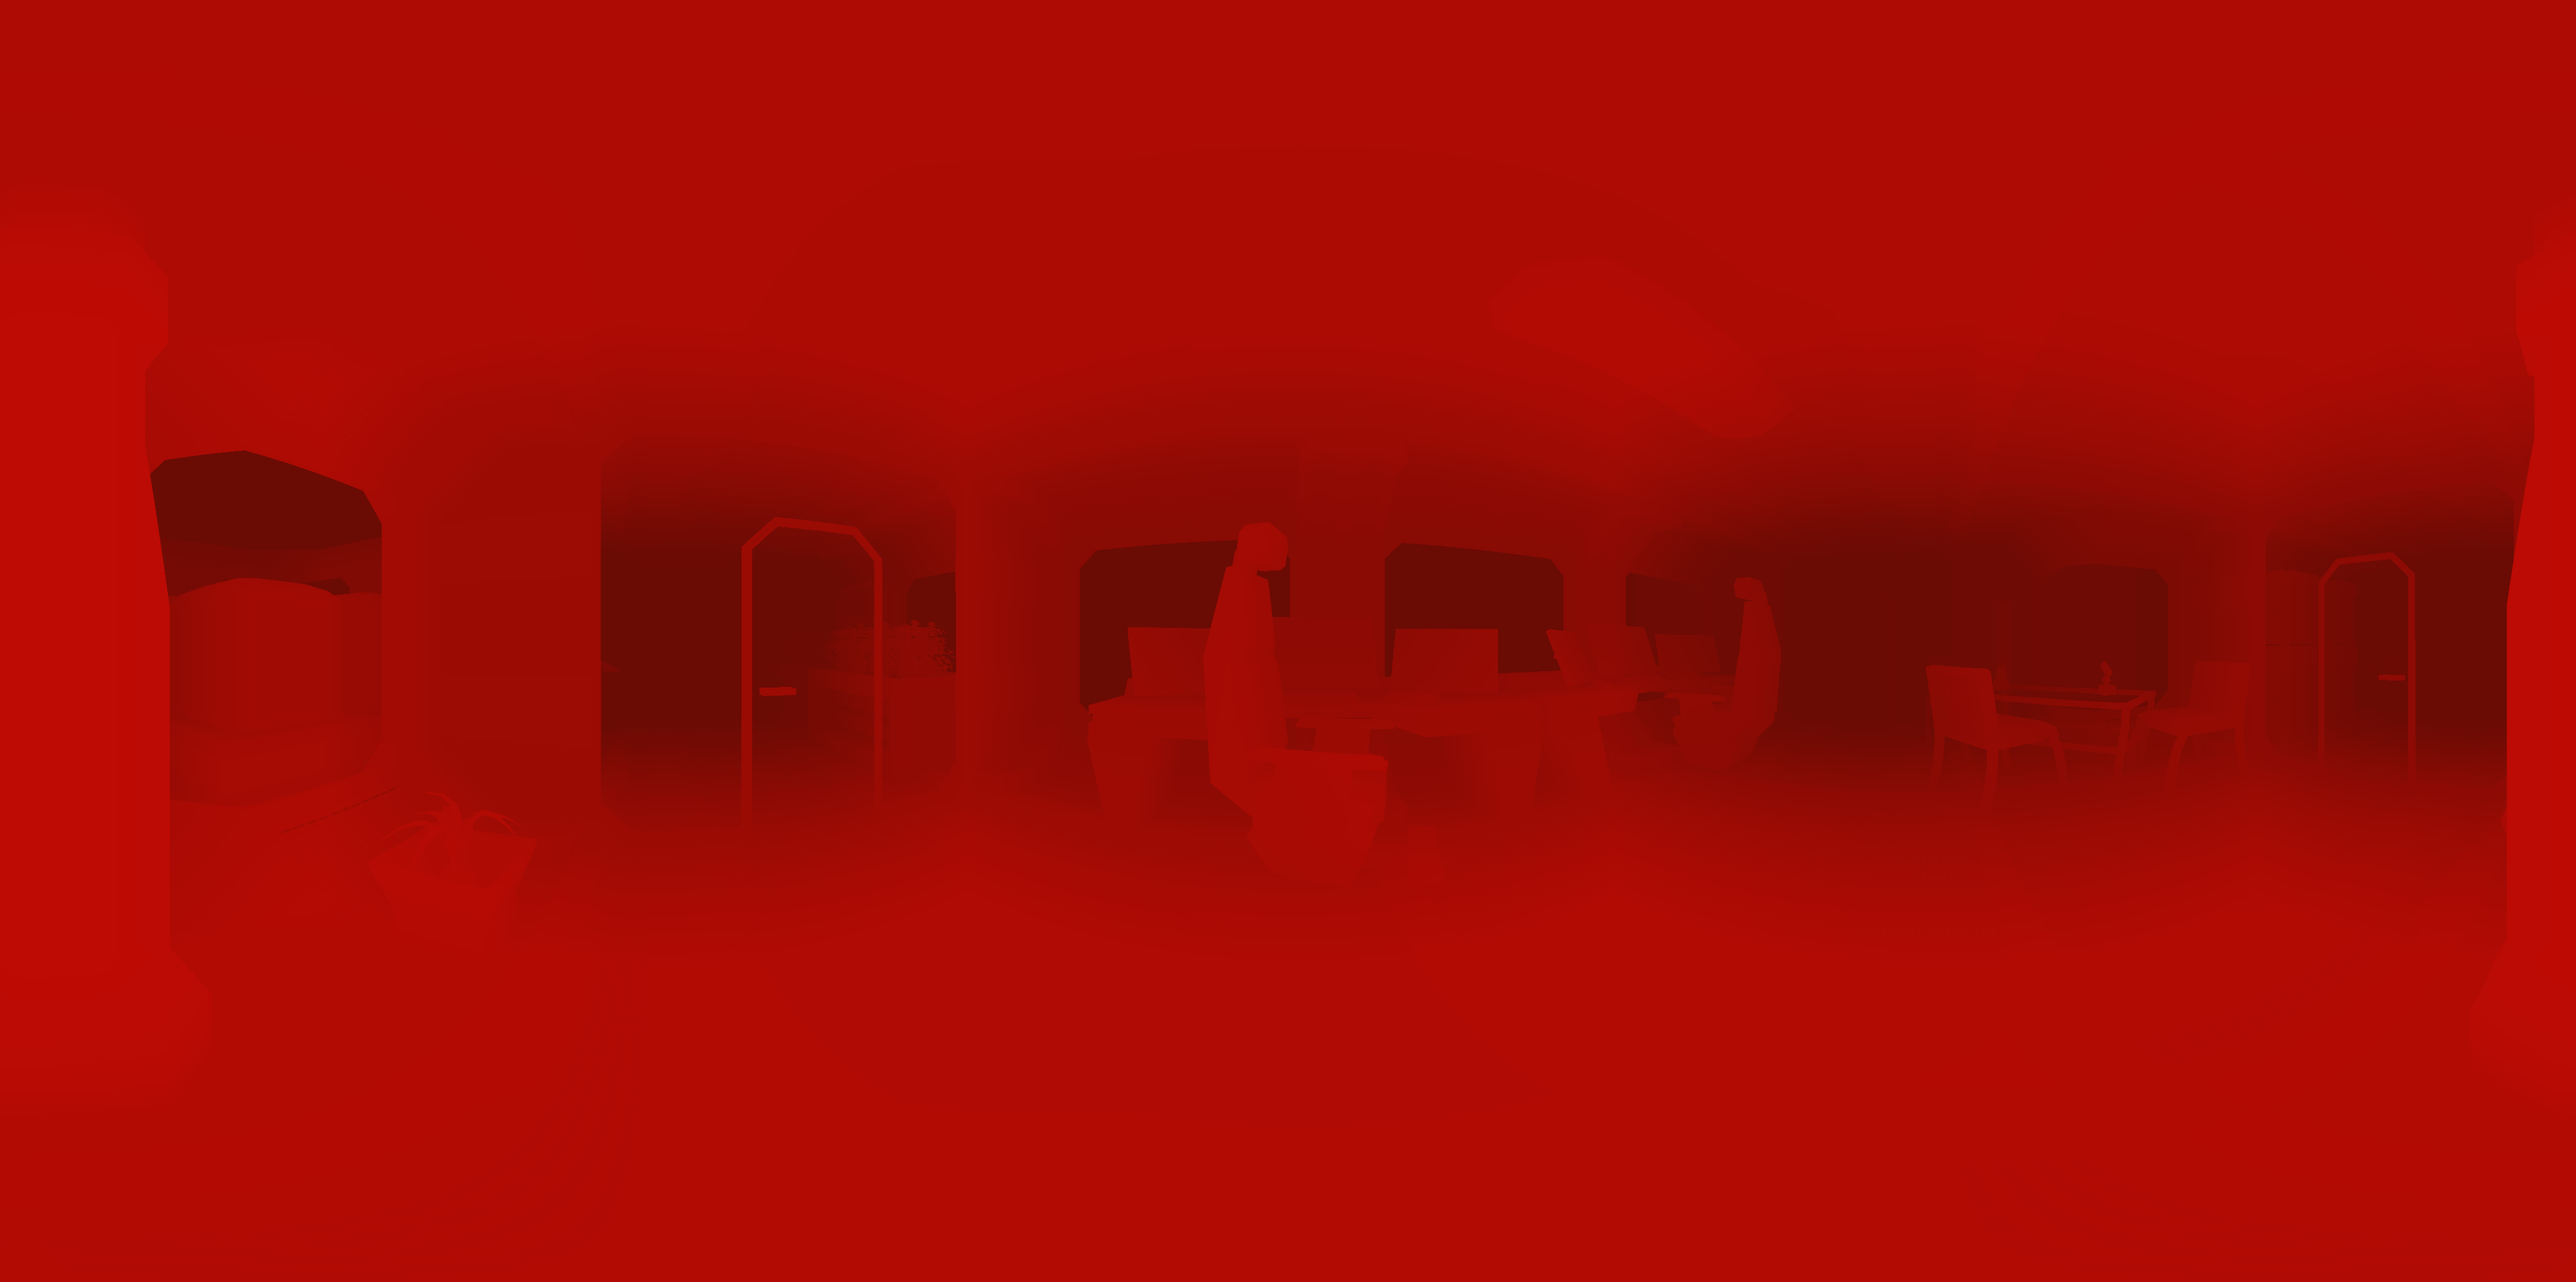
\includegraphics[width=0.7\textwidth]{red-depthmap-example}
  \caption{Mapa de profundidad guardado en la componente r de una textura ``\textit{ARGB32}''.}
  \label{fig:red-depthmap-encoded-example}
\end{figure}
\FloatBarrier

A continuación se guarda el estado de la escena y se configuran elementos como el ``\textit{Rendering Path}'' o las ``\textit{Clear Flags}'' para asegurar que las opciones por defecto no afectan al \textit{render}. Este \textit{shader} va a reemplazar todos los tipos de \textit{shader} que se encuentren en la escena, por lo que hay que repetir parte del \textit{shader} con diferentes opciones de ``\texttt{RenderType}''. Por último hay que reemplazar el \textit{shader} por defecto por este \textit{shader} con la instrucción 

\texttt{camera.SetReplacementShader(depthShader, ``RenderType'');}

y establecer los parámetros configurables del \textit{shader}. Para mejorar la calidad del mapa se define un parámetro para establecer una profundidad máxima, con el fin de evitar elementos cercanos con poca precisión, ya que es dónde más se va a apreciar el paralaje.

Por último y como se había dicho anteriormente, se restablecen los parámetros de la escena para evitar que afecte a otras tareas posteriores.

\section{Primera aproximación: Paralaje sencillo}
La primera aproximación que se realiza consiste en un paralaje sencillo. Para ello se crea una escena nueva en la que hay una cámara de realidad virtual, y una esfera muy grande con un shader, para imágenes y vídeo 360, sencillo del paquete: Google VR.

\subsection{Qué es el paralaje} 
Si un observador toma una foto y luego mueve la cámara hacia la derecha sin rotarla y toma otra foto, algunos objetos o parte de ellos que aparecían en la primera imagen, serán tapados por otros en la segunda imagen. Si se comparan ambas fotos tomando la primera como referencia, se puede apreciar que los objetos cercanos están aparente mente más desplazados en la segunda foto que los objetos lejanos. Esto esta causado porque el ojo humano y las cámaras utilizan una proyección en perspectiva.

Este fenómeno es llamado paralaje y puedes ver el ejemplo con tres fotos en \ref{fig:full-parallax}.

\begin{figure}[H]
\centering
\begin{subfigure}{.32\linewidth}
	\centering
  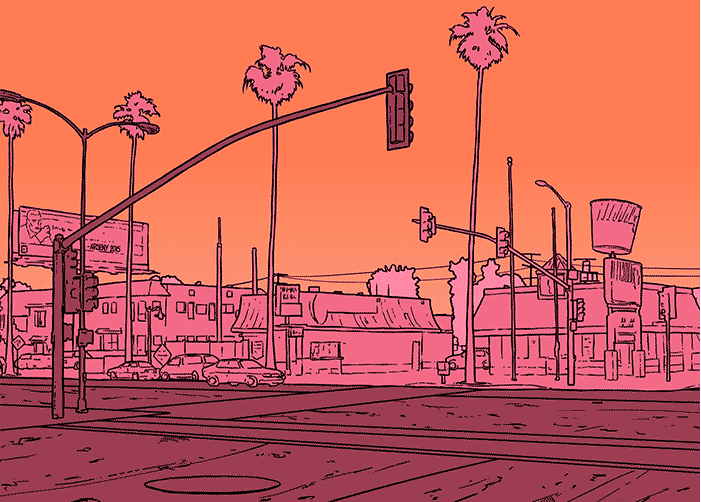
\includegraphics[width=\textwidth]{parallax-1}
  \caption{}
  \label{fig:parallax-1}
\end{subfigure}%
\hspace{.005\linewidth}
\begin{subfigure}{.32\linewidth}
	\centering
  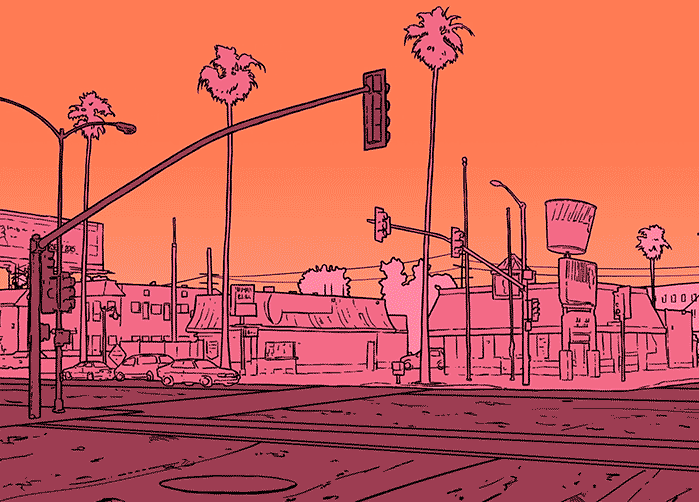
\includegraphics[width=\textwidth]{parallax-2}
  \caption{}
  \label{fig:parallax-2}
\end{subfigure}%
\hspace{.005\linewidth}
\begin{subfigure}{.32\linewidth}
	\centering
  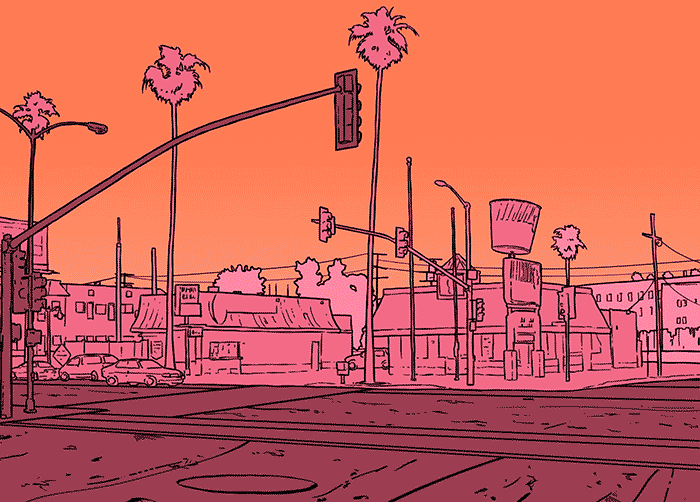
\includegraphics[width=\textwidth]{parallax-3}
  \caption{}
  \label{fig:parallax-3}
\end{subfigure}
\caption{Ejemplo de paralaje en tres fotogramas.}
\label{fig:full-parallax}
\end{figure}
\FloatBarrier


\subsection{Implementación} 
Es necesario hacer un paralaje en una imagen plana y para ello podemos mover píxeles por la superficie de la foto. Como se ha comentado en el apartado anterior, la cantidad que deben moverse los píxeles depende del dato obtenido del mapa de profundidades llevando a cabo una técnica similar a \cite{PedroParallax}.

La primera idea es modificar el \textit{shader} de visualización de vídeo y foto añadiéndole dos parámetros adicionales:

\begin{itemize}
\item \textit{Parallax Amount}: cuanto un píxel se debe desplazar teniendo en cuenta su profundidad.
\item \textit{Relative Position}: simula el desplazamiento de la cámara en el eje x en espacio de vista.
\end{itemize}

Estos parámetros se exponen con la finalidad de hacer una evaluación rápida de los resultados. Más adelante, la posición relativa será establecida mediante los datos que proporciona el casco de realidad virtual.

El \textit{shader} de vértices no es interesante para este caso, por lo tanto se va a comentar el \textit{shader} de fragmentos:

\begin{lstlisting}[language=glsl]
float4 frag (v2f i) : SV_Target {
  // Obteniendo la profundidad
  float h = DecodeFloatRGBA(tex2D(_DepthTex, i.uv));
  // Calculo del desplazamiento usando la profundidad.
  float uDisplacement = h * _ParallaxAmount 
                          * _RelativePosition 
                          * _DepthTex_TexelSize.x * 40;
  // Obteniendo el pixel de la posicion desplazada.
  return gammaCorrect(tex2D(_MainTex, 
               i.uv + float2(uDisplacement, 0)));
}
\end{lstlisting}

Cada píxel ``A'' en este caso, escoge el píxel ``B'' que se encuentra en la posición desplazada con respecto a la profundidad del píxel ``A'', esto quiere decir que el píxel ``B'' se está desplazando tanto como indica la profundidad de ``A''. Esto es una mala aproximación porque se tiene en cuenta la profundidad del píxel ``A'' y no el de ``B''.


\subsection{Resultado}
Como se ve en la figura \ref{fig:parallax-test-1}, se puede apreciar que los píxeles del fondo están siendo superpuestos sobre la silla y sin embargo, la silla no esta siendo desplazada sobre el fondo.

\begin{figure}[H]
  \centering
  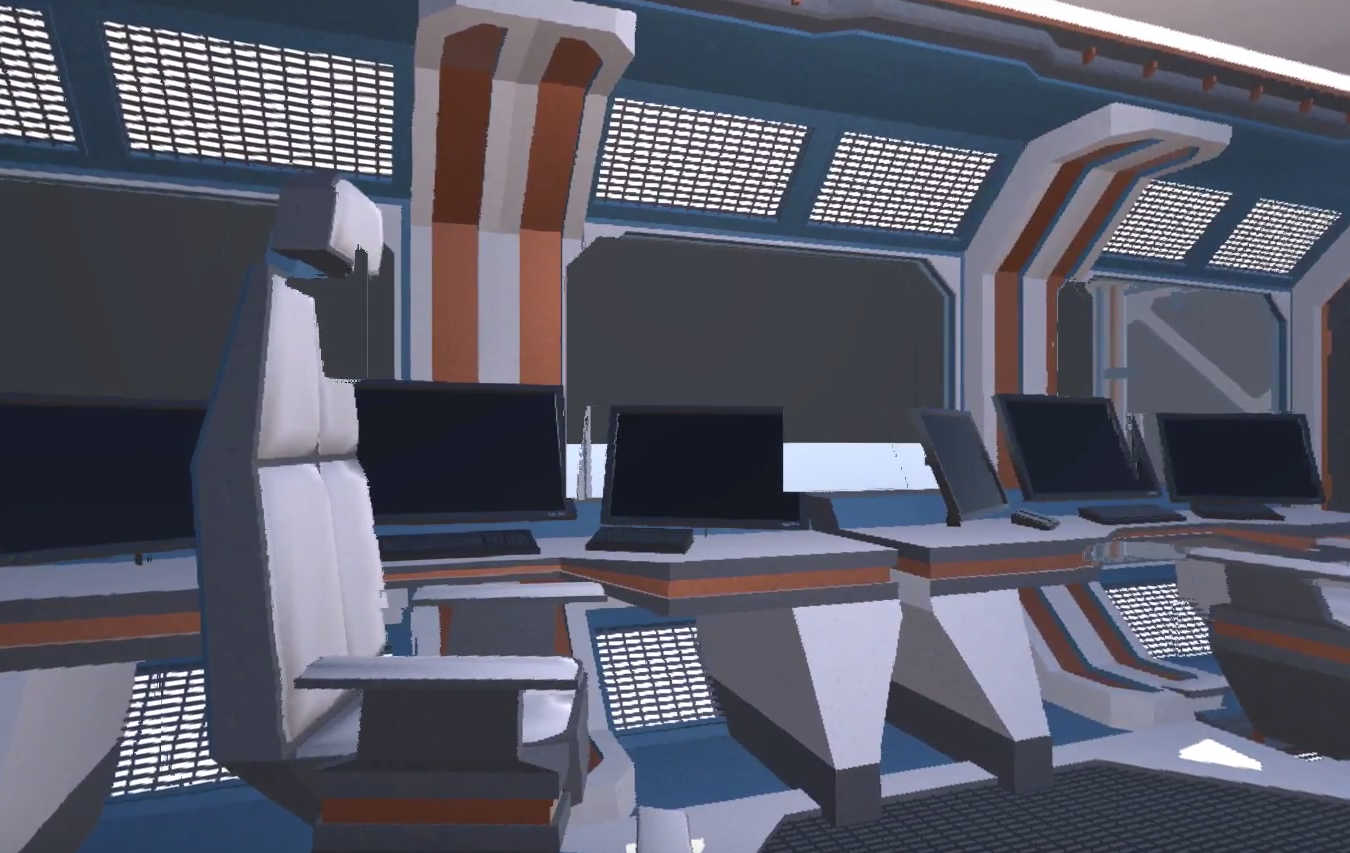
\includegraphics[width=0.9\textwidth]{parallax-test-1}
  \caption{Paralaje erróneo usando el desplazamiento equivocado.}
  \label{fig:parallax-test-1}
\end{figure}
\FloatBarrier

Se puede ver el vídeo en: \url{https://www.youtube.com/watch?v=F6zIchbR1Rg}

\section{Segunda aproximación: Paralaje sencillo}
El problema de la aproximación anterior era un mal planteamiento, debemos saber qué píxel B debe ocupar la posición del píxel A, pero la información para calcularlo, está en el píxel B. Por lo tanto para solucionar este problema de paralaje, la siguiente modificación del \textit{shader} realiza una búsqueda por la vecindad para encontrar cual es el mejor píxel para ocupar el actual.

\subsection{Implementación}
Esta idea realiza demasiados accesos a texturas y puede traer un problema muy grave de rendimiento. Sabiendo la dirección en la que se desplaza la cámara, sabemos la dirección en la que los píxeles se van a desplazar. De esta manera, simplificamos una búsqueda que implica un número de accesos a memoria cuadrático, en función de la distancia, a lineal.

Este es el nuevo \textit{shader} de fragmentos comentando las líneas principales.

\begin{lstlisting}[language=glsl]
float4 frag (v2f i) : SV_Target {
  // obtener la altura
  float height = DecodeFloatRGBA(tex2D(_DepthTex, i.uv));
  float maxHeight = 0;
  float2 bestUV = 0;
  float u = 0;
  bool found = false;
    
  // Dimension de texel con signo dependiendo
  // de la direccion de desplazamiento
  float texelSignedSize = sign(-_RelativePosition) 
                          * _DepthTex_TexelSize.x;
  // factor de desplazamiento
  float displacementFactor = _ParallaxAmount 
                            * -_RelativePosition 
                            * _DepthTex_TexelSize.x * 40;

  for (int itCount = 0; itCount < 40; itCount++) {
    // seleciona cada pixel en la linea elegida
    float2 currUV = i.uv + float2(u, 0);
    float currCellHeight = DecodeFloatRGBA(
                              tex2D(_DepthTex, currUV));
    float currCelluDispl = currCellHeight 
                           * displacementFactor;
    // calcular donde se deberia mover el pixel seleccionado
    float2 newUV = currUV + float2(currCelluDispl, 0);
        
    // si el pixel seleccionado esta en los limites 
    // del pixel actual, es un buen candidato
    if (abs(newUV.x - i.uv.x) <= _DepthTex_TexelSize.x) {
      // si es el pixel menos profundo, 
      // entonces es el mejor candidato hasta ahora
      if (currCellHeight >= maxHeight) {
        maxHeight = currCellHeight;
        bestUV = currUV;
        found = true;
      }
    }
    // pase de iteracion
    u -= texelSignedSize;
  }
    
  // si hay un buen candidato, pintalo
  // en otro caso, pinta en rosa
  return found ? gammaCorrect(tex2D(_MainTex, bestUV)) 
                : float4(1.0, 0.0, 1.0, 1.0);
}
\end{lstlisting}

\subsection{Resultado}
Esta aproximación es notablemente mejor, puesto que como se puede ver en \ref{fig:parallax-test-2}, los píxeles se desplazan en la dirección correcta, sin embargo se ve mucho ruido. Este ruido es causado las imágenes que son utilizadas, ya que en las opciones de Unity tiene se han activado tanto la compresión como el filtro bilinear.

\begin{figure}[H]
\centering
\begin{subfigure}{.47\linewidth}
	\centering
  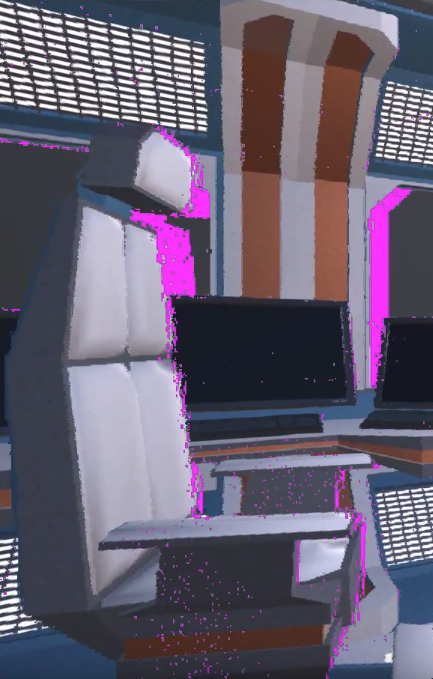
\includegraphics[width=\textwidth]{parallax-test-2-a}
  \caption{Relative position a 0.}
  \label{fig:parallax-test-2-a}
\end{subfigure}%
\hspace{.05\linewidth}
\begin{subfigure}{.47\linewidth}
	\centering
  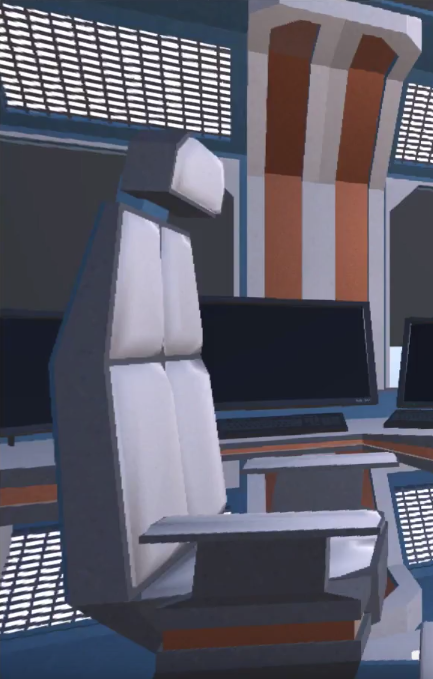
\includegraphics[width=\textwidth]{parallax-test-2-b}
  \caption{Relative position a 1.}
  \label{fig:parallax-test-2-b}
\end{subfigure}
\caption{Paralaje correcto con ruido.}
\label{fig:parallax-test-2}
\end{figure}
\FloatBarrier

Por simplicidad, se están utilizando accesos contiguos a textura y están ofreciendo un número alto de fotogramas por segundo. Si cambiamos el acceso añadiéndole otra dimensión de desplazamiento al \textit{shader}, los tiempos de acceso aumentarían mucho. Además el algoritmo no es escalable, pues cuanta más distancia haya que desplazar, más accesos son necesarios.

Se puede ver el vídeo en: \url{https://www.youtube.com/watch?v=wDxo_LH5Wjs}

\section{Tercera aproximación: Paralaje sencillo con \textit{shaders} de cómputo}
El último método da unos resultados razonablemente buenos pero el problema reside en el número de accesos a memoria hechos. 

Los \textit{shaders} gráficos tienen una limitación muy grande que consiste en que cada fragmento/píxel debe seleccionar su color, no puede pintar otro píxel del color indicado. Por este motivo se decide optar por los \textit{shaders} de cómputo.

\subsection{Implementación}
Esta idea realiza demasiados accesos a texturas y puede traer un problema muy grave de rendimiento. Sabiendo la dirección en la que se desplaza la cámara, sabemos la dirección en la que los píxeles se van a desplazar. De esta manera, simplificamos una búsqueda que implica un número de accesos a memoria cuadrático en función de la distancia a lineal.

Este es el nuevo \textit{shader} de fragmentos comentando las líneas principales. La ejecución consiste en una llamada al \textit{kernel} ``\textit{Clear}'' para limpiar los resultados y otra llamada al \textit{kernel} ``\textit{DisplaceAlbedo}''. El resultado se guarda en una \textit{RenderTexture} asociada al \textit{shader} gráfico básico de la esfera.

\begin{lstlisting}[language=glsl]
// Public kernels -----------------------
#pragma kernel Clear
#pragma kernel DisplaceAlbedo
#include "UnityCG.cginc"

// Config -------------------------------
// 360 stereo depth texture (IN)
Texture2D<fixed4> DepthTexture;
// 360 stereo albedo texture (IN)
Texture2D<fixed4> AlbedoTexture;
// 360 stereo computed result (OUT)
RWTexture2D<float4> Result;
// Los mismos parametros de configuracion 
// de los otros shader
float RelativePosition;
float ParallaxAmount;

// inicializar con rosa para ver los huecos
[numthreads(32, 32, 1)]
void Clear(uint3 id : SV_DispatchThreadID) {
    Result[id.xy] = float4(1.0f, 0.0f, 1.0f, -1.0f);
}

[numthreads(32, 32, 1)]
void DisplaceAlbedo (uint3 id : SV_DispatchThreadID) {
    // descodificar la altura
    float height = DecodeFloatRGBA(DepthTexture[id.xy]);
    // calculo de desplazamiento
    float displacementFactor = height 
                              * ParallaxAmount 
                              * RelativePosition;
                              
                              
    // aplicar el desplazamiento
    uint2 newUV = uint2(
                     (id.x + displacementFactor) % 4096, 
                     id.y);
    // devolver el albedo en la posicion calculada
    Result[newUV.xy] = float4(AlbedoTexture[id.xy].rgb, 1.0);
}
\end{lstlisting}

\subsection{Resultado}
Esta aproximación tiene un problema nuevo, que es el de concurrencia. Cuando un hilo calcula la nueva posición para escribir, muchos hilos pueden intentar escribir en la misma posición y el que termina escribiendo es uno aleatorio entre todos. Si eso ocurre, se ve algo parecido al ``\textit{z-fighting}'' que provoca el parpadeo de píxeles entre los diferentes colores que intenten ser escritos.

Como se puede ver en la figura \ref{fig:parallax-test-3}, las lineas negras señaladas con los círculos rojos, parpadean durante la ejecución.

\begin{figure}[H]
  \centering
  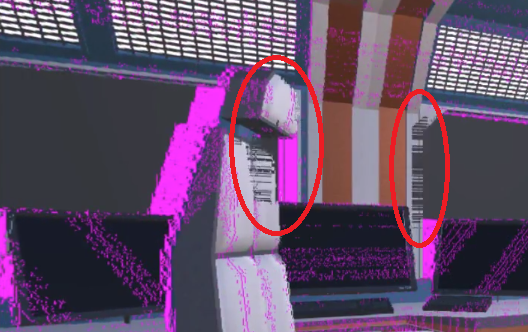
\includegraphics[width=0.5\textwidth]{parallax-test-3}
  \caption{Paralaje con condición de carrera.}
  \label{fig:parallax-test-3}
\end{figure}
\FloatBarrier

Se puede ver el vídeo en: \url{https://www.youtube.com/watch?v=R2rfZYyaCcE}

\section{Cuarta aproximación: Resolviendo la condición de carrera}
Para solucionar la condición de carrera la primera idea que surge es utilizar un \textit{z-buffer}.

\subsection{Implementación}
Para esta implementación, se pretende utilizar la instrucción \texttt{InterlockedMax} que asegura una escritura atómica del máximo entre la casilla seleccionada y el dato proporcionado a la función. Primeramente se utiliza una textura, pero esta instrucción no es compatible con texturas, por lo que se lleva a cabo con un \textit{buffer} lineal de int.

Por simiplificación, se eliminan las líneas ya explicadas en anteriores apartados. Esta vez se incorpora un nuevo \textit{kernel} llamado ``\textit{WriteDepth}'' que deberá ser llamado antes del ``\textit{DisplaceAlbedo}''

\begin{lstlisting}[language=glsl]
...
#pragma kernel WriteDepth
...
RWStructuredBuffer<int> Depth;
...
[numthreads(32, 32, 1)]
void Clear(uint3 id : SV_DispatchThreadID) {
    Result[id.xy] = float4(1.0f, 0.0f, 1.0f, -1.0f);
    Depth[bufferPos(id)] = -1;
}


uint bufferPos(uint3 id) {
    return id.x + id.y * 4096;
}


[numthreads(32, 32, 1)]
void WriteDepth(uint3 id : SV_DispatchThreadID) {
    float height = DecodeFloatRGBA(DepthTexture[id.xy]);
    float displacementFactor = height 
                              * ParallaxAmount 
                              * RelativePosition;
    uint2 newUV = uint2((id.x + displacementFactor) % 4096, 
                         id.y);
    int heightInt = height * 1024;

    // Se guarda la altura correcta en el buffer
    InterlockedMax(Depth[bufferPos(newUV)], 
                   heightInt);
    AllMemoryBarrier();
}

[numthreads(32, 32, 1)]
void DisplaceAlbedo(uint3 id : SV_DispatchThreadID) {
    int heightInt = Depth[bufferPos(id)];
    float height = (heightInt / 4096.0f);
    float displacementFactor = height 
                               * ParallaxAmount 
                               * -RelativePosition;
    uint2 newUV = uint2((id.x + displacementFactor) % 4096, 
                         id.y);


    // Se comprueba si la altura calculada
    // es la que debe usarse
    float3 albedoColor = heightInt == -1 ? 
                              float3(1.0f, 0.0f, 1.0f) : 
                              AlbedoTexture[newUV.xy].rgb;
    Result[id.xy] = float4(albedoColor, height);
}
\end{lstlisting}

\subsection{Resultado}
Este paralaje es el que mejor funciona hasta ahora como se puede ver en la figura \ref{fig:parallax-test-4}. El problema reside en que la función \textit{InterlockedMax} no esta estandarizada en todos los dispositivos. Además hay que llamar a tres \textit{kernels}, por lo que la cantidad de cálculos aumentan.

\begin{figure}[H]
  \centering
  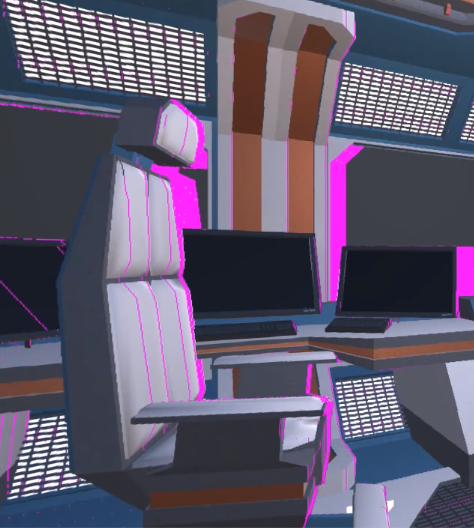
\includegraphics[width=0.5\textwidth]{parallax-test-4}
  \caption{Paralaje InterlockedMax.}
  \label{fig:parallax-test-4}
\end{figure}
\FloatBarrier

Se puede ver el vídeo en: \url{https://www.youtube.com/watch?v=MSG_IU-Xcjc}


\section{Quinta aproximación: Resolviendo la condición de carrera 2}
Llegados a este punto se opta por utilizar métodos más convencionales y se dejan sólo el kernel ``\textit{Clear}'' y ``\textit{DisplaceAlbedo}''.


\begin{lstlisting}[language=glsl]
...
[numthreads(32, 32, 1)]
void DisplaceAlbedo(uint3 id : SV_DispatchThreadID) {
  float height = DepthTexture[id.xy].r;
	float displacementFactor = (float)height 
	                            * (float)ParallaxAmount 
	                            * -RelativePosition;
	uint3 newUV = uint3(
	        (id.x + displacementFactor + 4096) % 4096, 
	         id.y, 
	         id.z);

  // Comprobar si se debe escribir muchas
  // veces para evitar sobreescrituras
	if ( Result[newUV.xy].a < DepthTexture[id.xy].r ) {
		Result[newUV.xy] = 
		    fixed4(AlbedoTexture[id.xy].rgb, 
		           DepthTexture[id.xy].r);
	}
	if ( Result[newUV.xy].a < DepthTexture[id.xy].r ) {
		Result[newUV.xy] = 
		    fixed4(AlbedoTexture[id.xy].rgb, 
		           DepthTexture[id.xy].r);
	}
	if ( Result[newUV.xy].a < DepthTexture[id.xy].r ) {
		Result[newUV.xy] = 
		    fixed4(AlbedoTexture[id.xy].rgb, 
		           DepthTexture[id.xy].r);
	}
	if ( Result[newUV.xy].a < DepthTexture[id.xy].r ) {
		Result[newUV.xy] = 
		    fixed4(AlbedoTexture[id.xy].rgb, 
		           DepthTexture[id.xy].r);
	}
	if ( Result[newUV.xy].a < DepthTexture[id.xy].r ) {
		Result[newUV.xy] = 
		    fixed4(AlbedoTexture[id.xy].rgb, 
		           DepthTexture[id.xy].r);
	}
}
\end{lstlisting}

\subsection{Resultado}
Este simple algoritmo elimina el parpadeo en un porcentaje muy alto, dando los mismos resultados que en el caso anterior. Además el rendimiento mejora con respecto a la versión de \textit{InterlockedMax}.

En estos momentos el \textit{shader} proporciona entre 160 y 180 fotogramas por segundo.


\section{Aproximación final: Pasando a espacio de mundo}
Hasta ahora todo lo que se había desarrollado era haciendo un desplazamiento de los elementos de la textura en la dimensión X. Esto es un desplazamiento falso, pues en un caso extremo podríamos tener delante de los ojos un elemento que se encuentre en nuestra espalda.

Para solucionar esto, se va a recalcular el desplazamiento en coordenadas de mundo.

\subsection{Implementación}
Para traducir a coordenadas de mundo hay que tener en cuenta que las dimensiones de la imagen están relacionadas con las coordenadas polares. Por lo tanto el orden de operaciones debería ser el siguiente:

\begin{enumerate}
\item Transformar de polares a cartesianas.
\item Desplazar las coordenadas cartesianas según el vector de desplazamiento indicado.
\item Transformar de cartesianas a polares.
\end{enumerate}

A continuación se puede ver la función que permite aplicar el desplazamiento. Hay muchas constantes nuevas que se utilizan para hacer los cálculos, algunas de ellas se podrían transformar en variables para ser modificadas externamente como la dimensión de la textura, pero para favorecer unas pruebas ágiles se considera innecesario.

\begin{lstlisting}[language=glsl]
static const float _PI = 3.14159265359;
static const float _2PI = 6.28318530718;
static const float _PI_2 = 1.57079632679;

static const uint2 TexDim = uint2(4096, 4096);
static const uint2 TexGrid = uint2(1, 2);
static const uint2 GridElemDim = uint2(4096, 2048);
static const uint FloatToUintDepthMultiplier = 4096;
static const float UintToFloatDepthMultiplier = 1.0/4096.0;

...

uint3 Displacement(uint2 id, 
                   float height, 
                   float3 displacementVector) {
                   
  // cambiar de altura a profundidad
  float depth = 1 - height;

  // id = ([0, 4095], [0, 2047])
  float2 onePixelInRadians = float2(_2PI, _PI) 
                             / (GridElemDim - 1);
                             
  // calcular radianes de coordenadas polares
  float2 theta_phi = (id.xy * onePixelInRadians) 
                     - float2(_PI, _PI_2);

  // calcular senos y cosenos de theta phi
  float2 sin_theta_phi = sin(theta_phi);
  float2 cos_theta_phi = cos(theta_phi);
    
    
    
  // pasar a coordenadas de mundo
  float3 worldPos = 
      float3(cos_theta_phi.y*sin_theta_phi.x, 
             sin_theta_phi.y,
             cos_theta_phi.y*cos_theta_phi.x) * depth;
             
  // desplazar las coordenadas en 
  // la direccion indicada
  worldPos += displacementVector;

  // calcular la nueva profundidad
  float newDepth = length(worldPos);
  // y normalizar la nueva posicion
  float3 newWorldNorm = worldPos / newDepth; 

  // calcular atan2 para pasar a polares
  float atan2ThetaPhi = atan2(newWorldNorm.x, 
                              newWorldNorm.z);

  // calcular coordenadas polares
  theta_phi = float2(atan2ThetaPhi, 
                     asin(newWorldNorm.y));
  theta_phi = (theta_phi / float2(_2PI, _PI) + 0.5) 
              * (GridElemDim - 1);

  // devolver las coordenadas polares
  // y la nueva profundidad
  return uint3(theta_phi, 
              (1-newDepth) * FloatToUintDepthMultiplier);
}


...

[numthreads(32, 32, 1)]
void WriteDepth(uint3 id : SV_DispatchThreadID) {
  float height = DepthTexture[id.xy].r;
  // calculamos el cuadrante
  uint2 quadrant = id.xy / GridElemDim;

  // Se aplica el desplazamiento
  uint3 newUV = Displacement(
                    uint2(id.x, id.y) % GridElemDim, 
                    height,
                    float3(ParallaxAmount * 
                            -RelativePosition, 
                           0, 0));
                           
  // devolvemos las uv a su cuadrante
  newUV.xy += quadrant * GridElemDim;
    
  // MULTIWRITE MODE
  if ( Result[newUV.xy].a < DepthTexture[id.xy].r ) {
    Result[newUV.xy] = fixed4(AlbedoTexture[id.xy].rgb, 
                              DepthTexture[id.xy].r);
  }
  ... // x5
}

\end{lstlisting}

\subsection{Resultado}

Como se puede observar en \ref{fig:parallax-test-5-12} y \ref{fig:parallax-test-5-35}, el desplazamiento producido es bastante realista, pero deja demasiados huecos rosas.

Este \textit{shader} reduce el número de fotogramas por segundo un poco, dejándolo en aproximadamente 140-160 fotogramas por segundo.

\begin{figure}[H]
\centering
\begin{subfigure}{.47\linewidth}
	\centering
  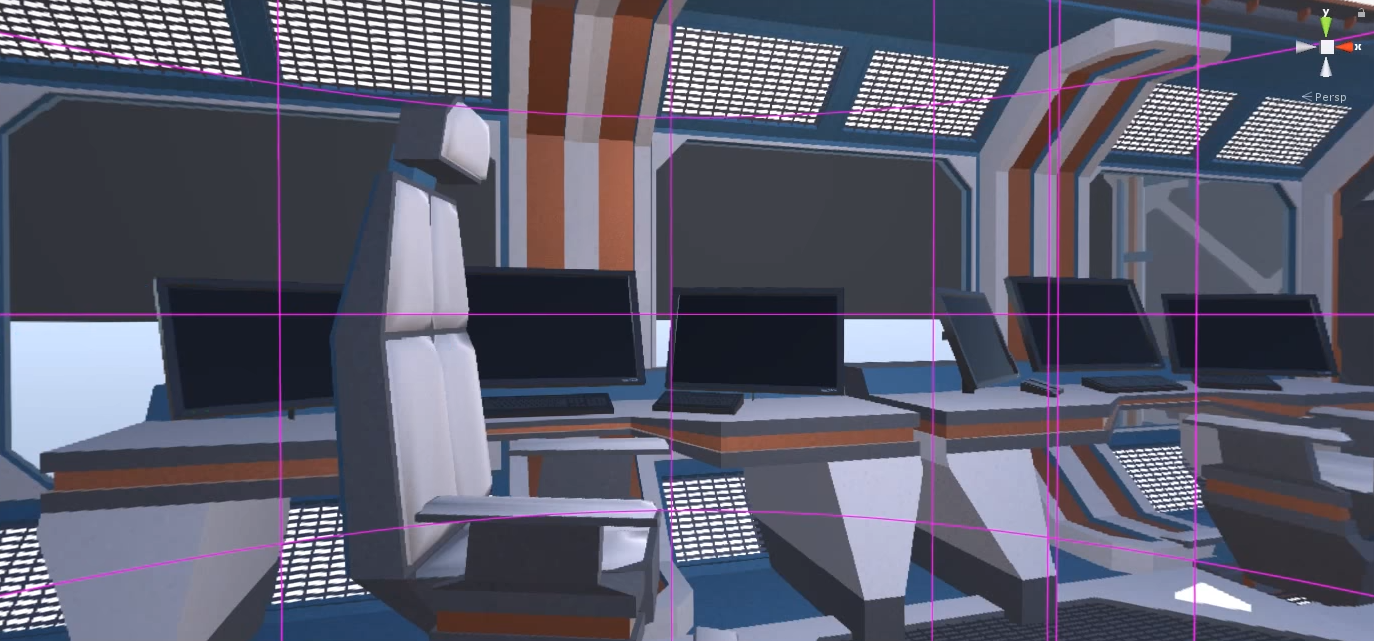
\includegraphics[width=\textwidth]{parallax-test-5-1}
  \caption{}
  \label{fig:parallax-test-5-1}
\end{subfigure}%
\hspace{.05\linewidth}
\begin{subfigure}{.47\linewidth}
	\centering
  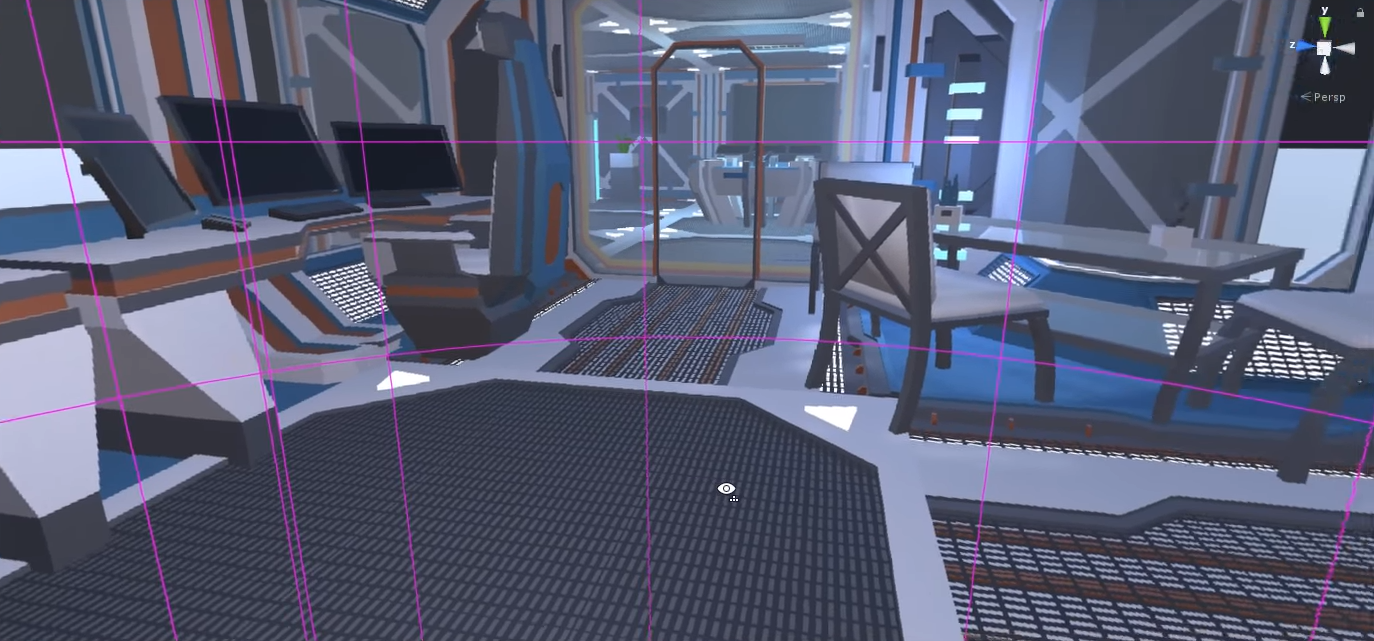
\includegraphics[width=\textwidth]{parallax-test-5-2}
  \caption{}
  \label{fig:parallax-test-5-2}
\end{subfigure}
\caption{Sin desplazamiento.}
\label{fig:parallax-test-5-12}
\end{figure}

\begin{figure}[H]
\centering
\begin{subfigure}{.47\linewidth}
	\centering
  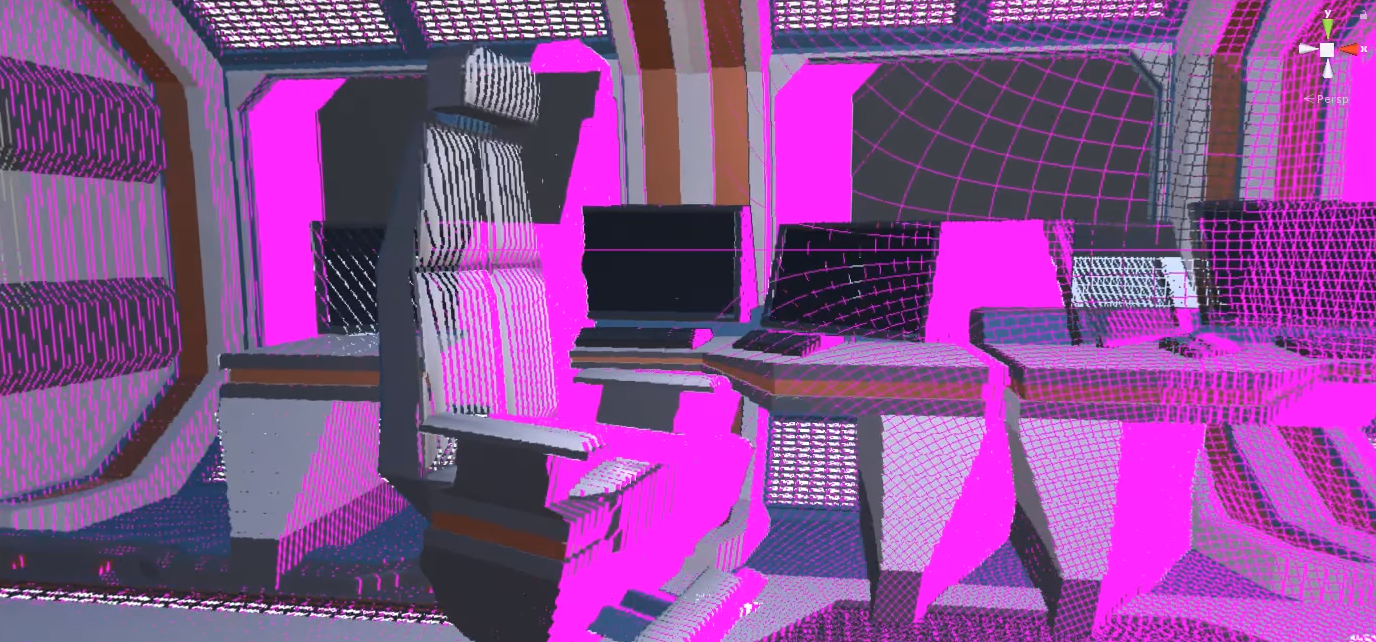
\includegraphics[width=\textwidth]{parallax-test-5-3}
  \caption{}
  \label{fig:parallax-test-5-3}
\end{subfigure}%
\hspace{.05\linewidth}
\begin{subfigure}{.47\linewidth}
	\centering
  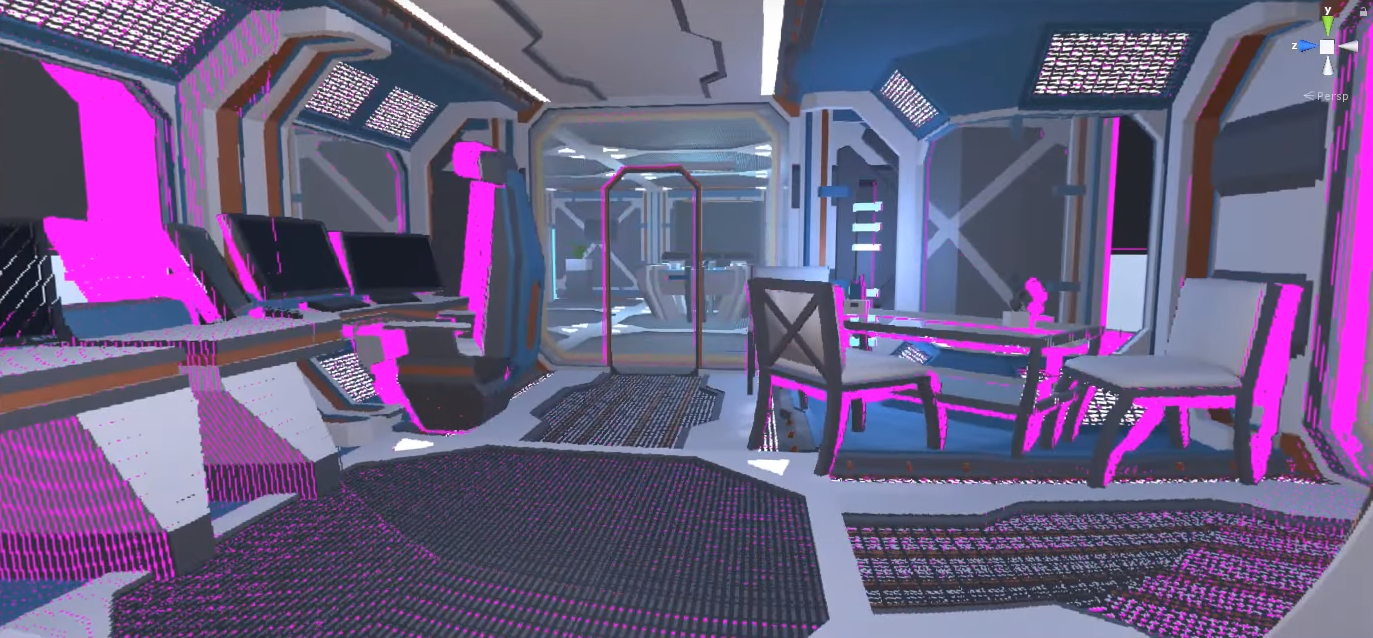
\includegraphics[width=\textwidth]{parallax-test-5-5}
  \caption{}
  \label{fig:parallax-test-5-5}
\end{subfigure}
\caption{Con el máximo desplazamiento.}
\label{fig:parallax-test-5-35}
\end{figure}
\FloatBarrier

Se puede ver el vídeo en: \url{https://www.youtube.com/watch?v=vdR3ZlCLFCQ}


\section{Otras pruebas}

\subsection{Evitar borrar el \textit{buffer} de color}
Además de lo visto en el \textit{shader}, se han realizado pruebas limpiando únicamente el \textit{buffer} de profundidad que actualmente es la componente \textit{alpha} de la textura de resultados. Estas pruebas evitan la aparición de elementos rosas y rellena con el último color que tuvo esa textura. 

Esto da resultados visualmente muy buenos, pues los píxeles vacíos provocados por un estiramiento de la textura, son tapados automáticamente. No da tan buen resultado con los grandes huecos provocados por saltos de profundidad.

\begin{figure}[H]
\centering
\begin{subfigure}{.47\linewidth}
	\centering
  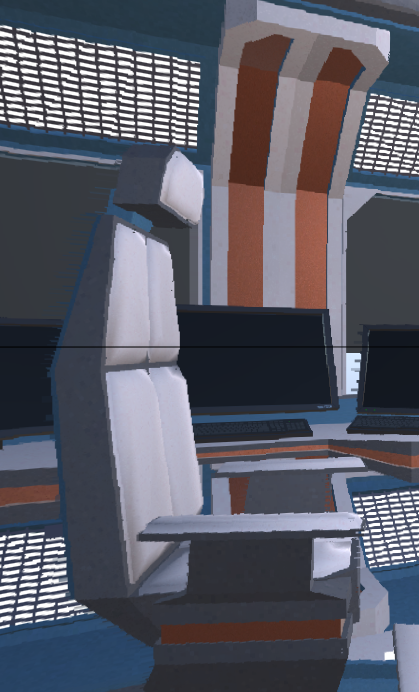
\includegraphics[width=\textwidth]{parallax-test-5a}
  \caption{}
  \label{fig:parallax-test-5-a}
\end{subfigure}%
\hspace{.05\linewidth}
\begin{subfigure}{.47\linewidth}
	\centering
  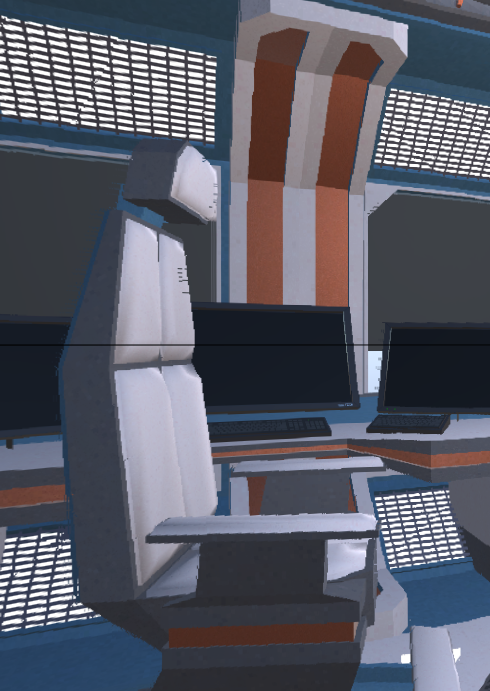
\includegraphics[width=\textwidth]{parallax-test-5b}
  \caption{}
  \label{fig:parallax-test-5-b}
\end{subfigure}
\caption{Desplazamiento sin borrar el color.}
\label{fig:parallax-test-5ab}
\end{figure}

\begin{figure}[H]
\centering
\begin{subfigure}{.47\linewidth}
	\centering
  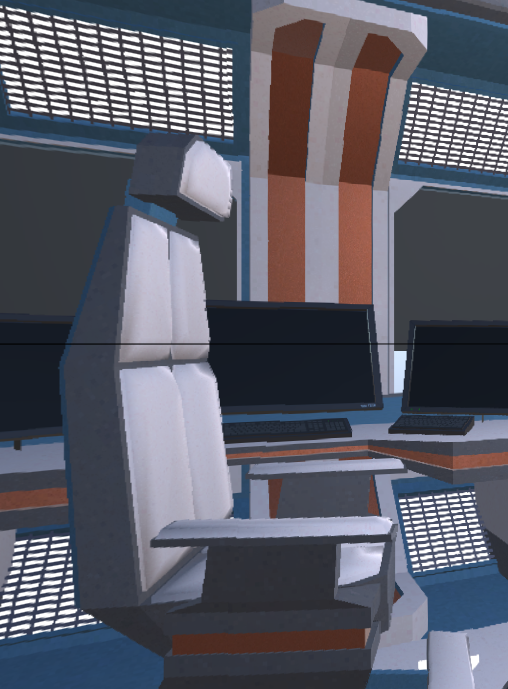
\includegraphics[width=\textwidth]{parallax-test-5c}
  \caption{}
  \label{fig:parallax-test-5-c}
\end{subfigure}%
\hspace{.05\linewidth}
\begin{subfigure}{.47\linewidth}
	\centering
  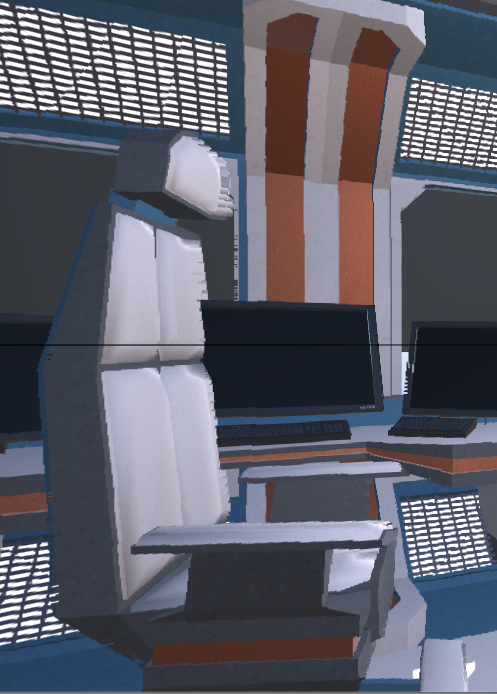
\includegraphics[width=\textwidth]{parallax-test-5d}
  \caption{}
  \label{fig:parallax-test-5-d}
\end{subfigure}
\caption{Desplazamiento sin borrar el color.}
\label{fig:parallax-test-5cd}
\end{figure}
\FloatBarrier

\subsection{Desplazamiento en espacio de mundo con shaders gráficos}
Se han realizado pruebas aplicando la lógica de desplazamiento en espacio de mundo a un \textit{shader} gráfico. Al no poder aprovechar la ventaja de saber en que dirección buscar el píxel apropiado, la búsqueda realizada debía ser cuadrática y el rendimiento bajaba en un ordenador de sobremesa con tarjeta gráfica de última generación por debajo de los 30 fotogramas por segundo con un \textit{kernel} de búsqueda de 40x40, dando además un resultado con grandes cantidades de píxeles perdidos.

\subsection{Completar con el ojo opuesto}
Una de las propuestas para mejorar este algoritmo, es utilizar la textura del ojo opuesto como herramienta para rellenar huecos, que de otra manera quedarían vacíos, utilizando las mismas operaciones que se venían usando, pero aplicando pequeñas modificaciones para el nuevo ojo. Se ha realizado un esbozo de esta tecnología pero no se ha podido llevar a cabo por falta de tiempo.





